\documentclass[12pt]{article}


\begin{document}
La fabrication des formes géometriques dans ce projet a pour but de donner la possibilité aux utilisateurs de construire les formes qu'ils souhaitent.
Il existe 5 formes dans notre projet, chaque forme a sa propre classe. On a donc la classe Rectangle, PyramideTriangulaire, Pyramide, Prism et Icosphere.
Ces classes extend la classe ShapeTriangleUtil qui factorise les méthodes communes aux Shape "faites avec des triangles"  et  implémentent la classe Shape qui est l'interface pour définir une forme.

\begin{figure}[ht]
\begin{center}
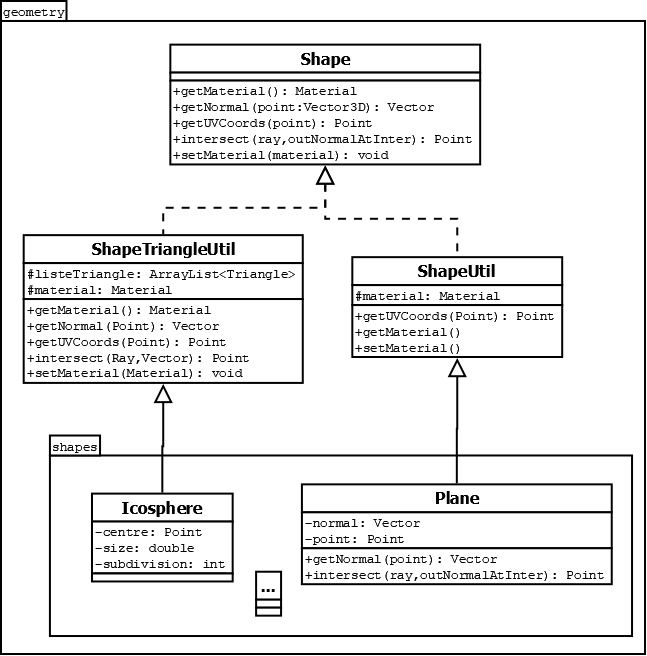
\includegraphics[scale=\umlscale]{./diagrammes/package_geometry.png}
\caption{Diagramme d'h\'eritage des classes}
\end{center}
\end{figure}

\end{document}